% Partie devenir sponsor

Capitole du Libre recherche des partenaires financer l'événement et que l'évenment reste libre et accessible au plus grand nombre de personnes. Nous proposons à tout type d'entreprises de nous aider avec différents niveaux de sponsorins détaillés ci-dessous.

\Separateur

Nous sponsoriser, c'est vous associer à cette manifestation et contribuer au Logiciel Libre. Capitole du Libre est un lieu idéal pour venir découvrir de nouveaux horizons, récolter de nouvelles idées, découvrir de nouveaux talents

	\subsection{Niveaux de sponsoring}

    \begin{center}
    \begin{tabular}{|r|c|c|c|c|c|}
        \hline  & Bronze & Argent & Or & Platine & Diamant \\
        \hline Contribution & \SI{250}{\euro} & \SI{600}{\euro} & \SI{1000}{\euro} & \SI{2000}{\euro} & \SI{3000}{\euro} \\
        \hline Limite & - & - & - & 4 & 2 \\
        \hline Logo sur l'affiche et le site web & \ding{'064} & \ding{'064} & \ding{'064} & \ding{'064} & \ding{'064}  \\
        \hline Badges sponsors & \ding{'064} & \ding{'064} & \ding{'064} & \ding{'064} & \ding{'064} \\
        \hline Dépôt d'offre d'emploi et de stage & \ding{'064} & \ding{'064} & \ding{'064} & \ding{'064} & \ding{'064} \\
        \hline Logo diffusé entre les conférences & & \ding{'064} & \ding{'064} & \ding{'064} & \ding{'064} \\
        \hline Logo au début de chaque vidéo & & & \ding{'064} & \ding{'064} & \ding{'064} \\
        \hline Logo sur les \textit{flyers} de l'événement & & & \ding{'064} & \ding{'064} & \ding{'064} \\
        \hline Texte sur le programme distribué & & & \nicefrac{1}{4} page & \nicefrac{1}{2} page & 1 page \\
        \hline Stand à proximité des buvettes & & & & 1 table & 2 tables \\
        \hline Remerciements lors de la conférence de clôture & & & & \ding{'064} & \ding{'064}  \\
        \hline Une idée ? Contactez-nous ! & & & & & \ding{'064} \\
        \hline Mise à disposition d'une salle privative & & & & & \ding{'064} \\
        \hline 
    \end{tabular}
    \end{center}

Note: sur les différents supports, la taille de votre logo sera proportionnelle à votre niveau de support.

	\subsection{Retour d’expérience des précédents \textit{sponsors}}
	\subsection{Budget de l’événement}

Le budget total de l'édition 2014 de Capitole du Libre s'élevait à \SI{12000}{\euro}. Les différents postes de dépense sont indiqués dans le graphique ci-dessous:

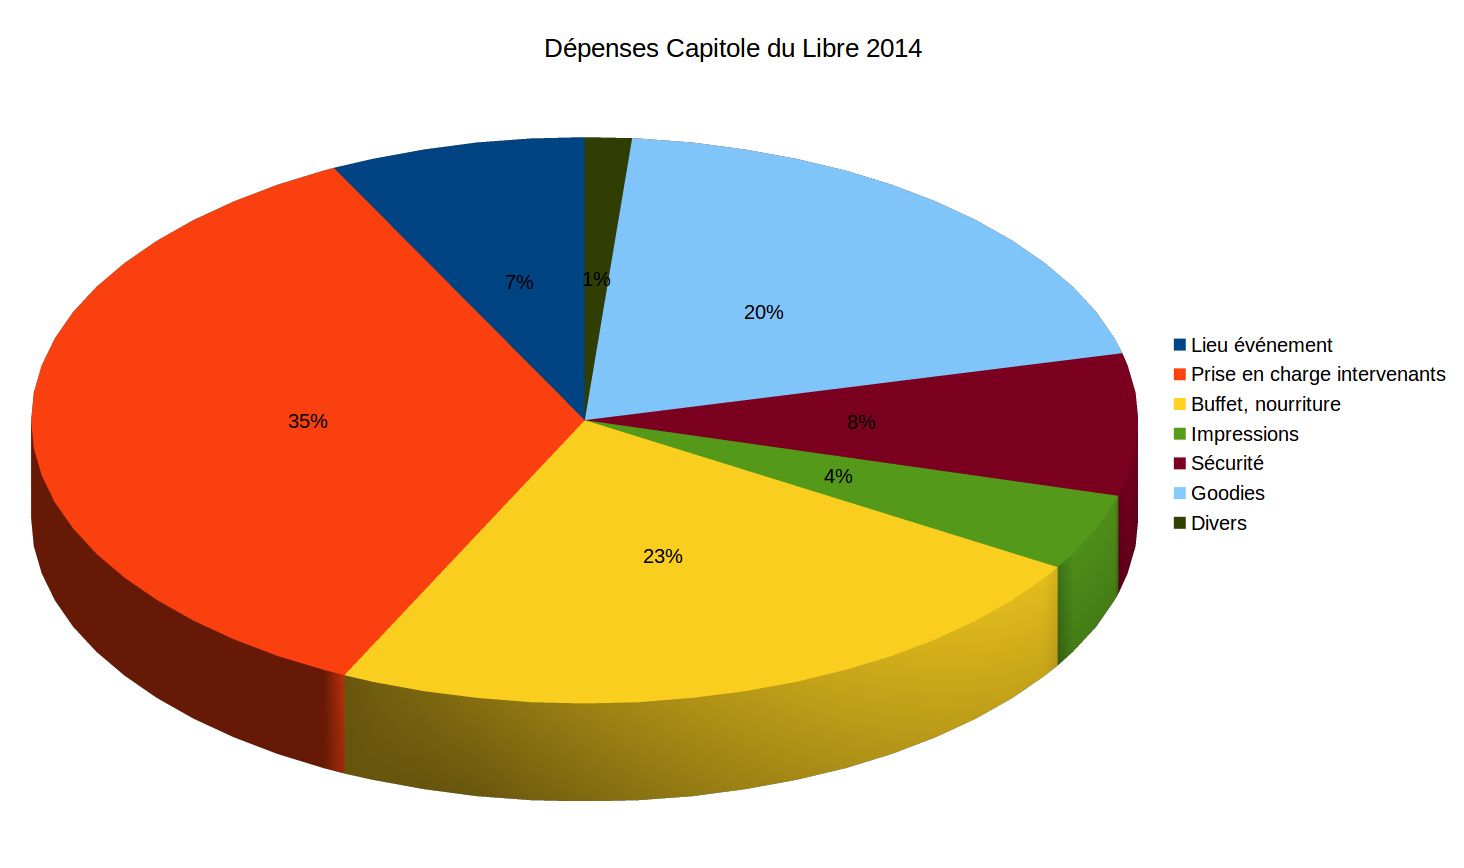
\includegraphics[scale=0.6]{Images/budget_2014.png}\\

Pour l'édition 2015 de Capitole du Libre, nous prévoyons une augmentation de notre budget à \SI{18000}{\euro} afin principalement :
\begin{itemize}[label=$\bullet$]
\item de permettre de faire venir plus d'orateurs de plus loin afin de continuer à améliorer la qualité et la variété de nos orateurs ;
\item de réaliser un buffet correct le samedi soir (l'année dernière nous avions été vraiment trop juste en quantité). Ce buffet ouvert à tous et à participation libre étant un lieu d'échange privilégié lors de ce week-end où se retrouvent orateur et participants des différentes thématiques.
\end{itemize}

\Separateur

Le détail des dépenses de Capitole du Libre 2015 est détaillé dans le tableau ci-dessous:

\begin{center}
    \begin{tabular}{|l|c|}
        \hline Dépense & Montant \\
        \hline \textbf{Défraiements intervenants} & \textbf{\SI{5000}{\euro}} \\
        \hline Déplacements intervenants & \SI{3500}{\euro} \\
        \hline Hébergement intervenants & \SI{1500}{\euro} \\
        \hline \textbf{Hébergement manifestation} & \textbf{\SI{3000}{\euro}}\\
        \hline Chauffage & \SI{1500}{\euro} \\
        \hline Sécurité & \SI{1500}{\euro} \\
        \hline \textbf{Apéritif \& Repas} & \textbf{\SI{6000}{\euro}}\\
        \hline Participation repas intervenants et bénévoles & \SI{1500}{\euro} \\
        \hline Buffet samedi soir & \SI{4500}{\euro} \\
        \hline \textbf{Buvette} & \textbf{\SI{600}{\euro}}\\
        \hline Viénoiseries bénévoles & \SI{150}{\euro} \\
        \hline Approvisionnement buvette & \SI{400}{\euro} \\
        \hline Location machines à café & \SI{50}{\euro} \\
        \hline \textbf{Goodies} & \textbf{\SI{2800}{\euro} }\\
        \hline T-Shirt Capitole du Libre 2015 & \SI{1400}{\euro} \\
        \hline Goodies autres & \SI{1400}{\euro} \\
        \hline \textbf{Communication} & \textbf{\SI{800}{\euro}} \\
        \hline Impression Flyyers & \SI{100}{\euro} \\
        \hline Impression Affiches & \SI{100}{\euro} \\
        \hline Impression Programmes & \SI{500}{\euro} \\
        \hline Fléchage / Indications & \SI{100}{\euro} \\
        \hline
        \hline TOTAL & \SI{18200}{\euro} \\
        \hline
    \end{tabular}
\end{center}

\Separateur

Les recettes 2015 sont détaillées dans le tableau ci-dessous:

\begin{center}
    \begin{tabular}{|c|c|c|c|c|c|}
        \hline Dépense & Montant \\
        \hline Sponsors & \SI{15900}{\euro} \\
        \hline Dons & \SI{300}{\euro} \\
        \hline Ventes buvette & \SI{600}{\euro} \\
        \hline Recette boutique & \SI{1600}{\euro} \\
        \hline TOTAL & \SI{18200}{\euro} \\
        \hline
    \end{tabular}
\end{center}

